\documentclass[11pt]{article}
\usepackage[margin=20mm]{geometry}
\usepackage{amsmath}
\usepackage{float}
\usepackage{subfig}
\usepackage{listings,color,enumitem}
\definecolor{mygreen}{RGB}{28,172,0} % color values Red, Green, Blue
\definecolor{mylilas}{RGB}{170,55,241}
\usepackage{graphicx}

%\graphicspath{results/}
\title{Homework 4\\ \vspace{2mm}\Large{16-720A Computer Vision }}
\author{Matthew Swenson}

\begin{document}
	\maketitle
	
\section*{Q 1.1}
We know 
$$pFp'=0$$
Given the problem constraint that both points in question lie at $(0,0)$ on their camera planes, we can write
$$
\begin{bmatrix}0 &0& 1\end{bmatrix}
\left[\begin{array}{ccc} f_{1,1} & f_{1,2} & f_{1,3}\\ f_{2,1} & f_{2,2} & f_{2,3}\\ f_{3,1} & f_{3,
2} & f_{3,3} \end{array}\right]
\begin{bmatrix}0\\ 0\\ 1\end{bmatrix}
    =
    0
$$
$$
\begin{bmatrix}f_{3,1} &f_{3,2}& f_{3,3}\end{bmatrix}
\begin{bmatrix}0\\ 0\\ 1\end{bmatrix}
    =
    0
$$
$$f_{3,3}  = 0$$

\section*{Q 1.2}
Given the formula for the coefficients of an epipolar line: $l = \mathcal{E}*p'$ and the formula for the essential matrix: $\mathcal{E}=[t_\times]R$, the knowledge
that $t = \begin{bmatrix}x &0& 0\end{bmatrix}$ and $R=I$, because there is only x-axis translation:
$$\mathcal{E}={t_\times}R = 
\begin{bmatrix}0 &-t_3& t_2\\ t_3 & 0& -t_1 \\-t_2 &t_1& 0\end{bmatrix}I =
\begin{bmatrix}0 &0& 0\\ 0& 0&-x \\0 &x& 0\end{bmatrix}
    $$
    $$l=
\begin{bmatrix}0 &0& 0\\ 0& 0&-x \\0 &x& 0\end{bmatrix}
\begin{bmatrix}a\\ b\\ c\end{bmatrix}
    =
\begin{bmatrix}0\\-xc\\ xb\end{bmatrix}
    $$
    Because the resulting line coefficients have 0 for their X component, the line must be parallel to the x axis.
\section*{Q 1.3}
$$R_{rel}=R_i$$
$$t_{rel}=t_i$$
$$\mathcal{E}=[t_{rel_\times}]R_{rel}$$
$$F=K^{-T}\mathcal{E}K^{-1}$$
\section*{Q 1.4}
The plane of the mirror is functionally equivalent to the image plane of a different camera. Because it has
no real camera center but is being obeserved by the current camera, we can treat the mirror as having the same
intrinsic matrix as the real camera. To find its center, define the translation from the real camera's
center to its image plane, and the translation and rotation from the real camera image plane to the mirror. Composing 
these movements gives us the "center" of the mirror "camera". Because the mirror is a projecction plane
and we have an $R$ and $t$, we can define the essential and fundamental matrices as we normally would, 
therefore creating a skew symmetric fundamental matrix.

\section*{Q 2.1}
    $$F=\left(\begin{array}{ccc} -1.4444E{10}^{-9} & -7.8627E{10}^{-8} & 0.0011327\\ -1.1205E{10}^{-7} &
1.2618E{10}^{-9} & 4.1543E{10}^{-6}\\ -0.0010881 & 0.000015377 & -0.0046423 \end{array}\right)$$
\begin{figure}[H]
    \centering
    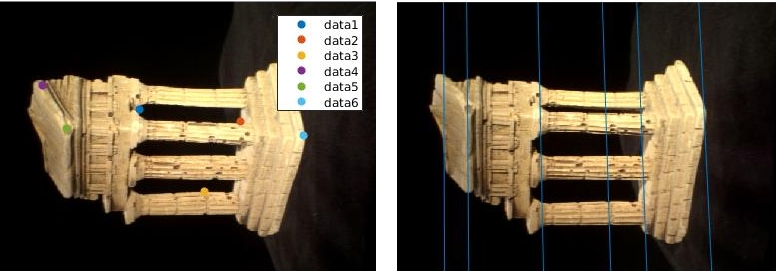
\includegraphics[width=\textwidth]{q2_1.jpg}
\end{figure}

\section*{Q 2.2}
    $$F=\left(\begin{array}{ccc} 3.0708E{10}^{-8} & 3.5025E{10}^{-7} & 0.0016039\\ -1.5483E{10}^{-7} & 9.
2714E{10}^{-9} & 0.000054917\\ -0.0016465 & -0.000030733 & -0.0091395 \end{array}\right)$$
\begin{figure}[H]
    \centering
    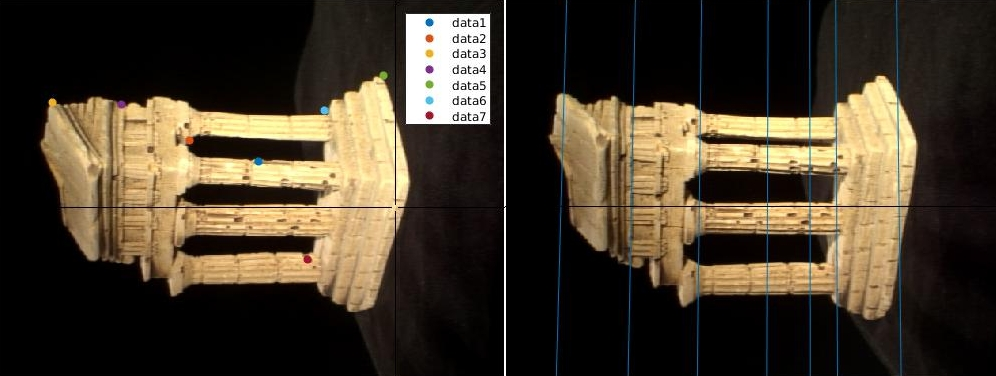
\includegraphics[width=\textwidth]{q2_2.jpg}
\end{figure}
\section*{Q 3.1}
    $$E=\left(\begin{array}{ccc} -0.0033389 & -0.18241 & 1.692\\ -0.25994 & 0.002938 & -0.044874\\ -1.6971 &
 -0.012332 & -0.00062738 \end{array}\right)$$
\section*{Q 3.2}
Given points $p_1 =[x_1\ y_1]$ and $p_2 =[x_2\ y_2]$ and camera matrices $C_1$ and $C_2$: 
\begin{align}
A =\begin{bmatrix}
       \begin{bmatrix}0& 0& 1\end{bmatrix} C_1*x_1 - \begin{bmatrix}1& 0& 0\end{bmatrix} C_1\\
       \begin{bmatrix}0& 0& 1\end{bmatrix} C_1*y_1 - \begin{bmatrix}0& 1& 0\end{bmatrix} C_1\\
       \begin{bmatrix}0& 0& 1\end{bmatrix} C_1*x_2 - \begin{bmatrix}1& 0& 0\end{bmatrix} C_2\\
       \begin{bmatrix}0& 0& 1\end{bmatrix} C_1*y_2 - \begin{bmatrix}0& 1& 0\end{bmatrix} C_2\\
   \end{bmatrix}
\end{align}
\section*{Q 4.1}
\begin{figure}[H]
    \centering
    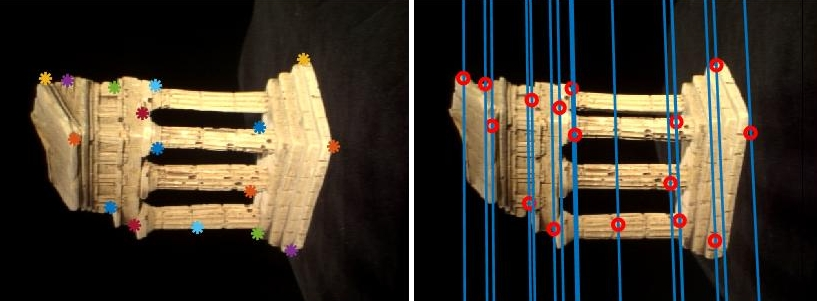
\includegraphics[width=\textwidth]{q4_1.jpg}
\end{figure}
\section*{Q 4.2}
\begin{figure}[H]
   %\centering
 \begin{tabular}{cc}
    \subfloat[]{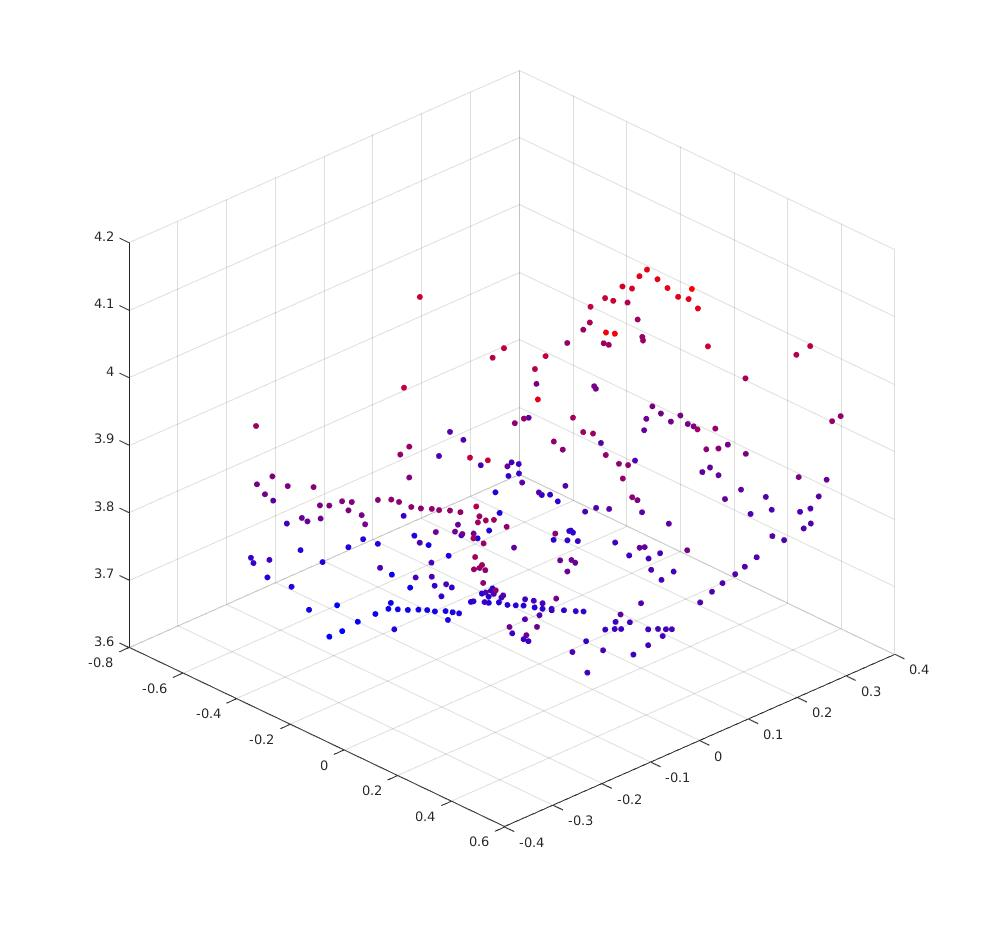
\includegraphics[width=.5\textwidth]{q4_2_1.jpg}} &
    \subfloat[]{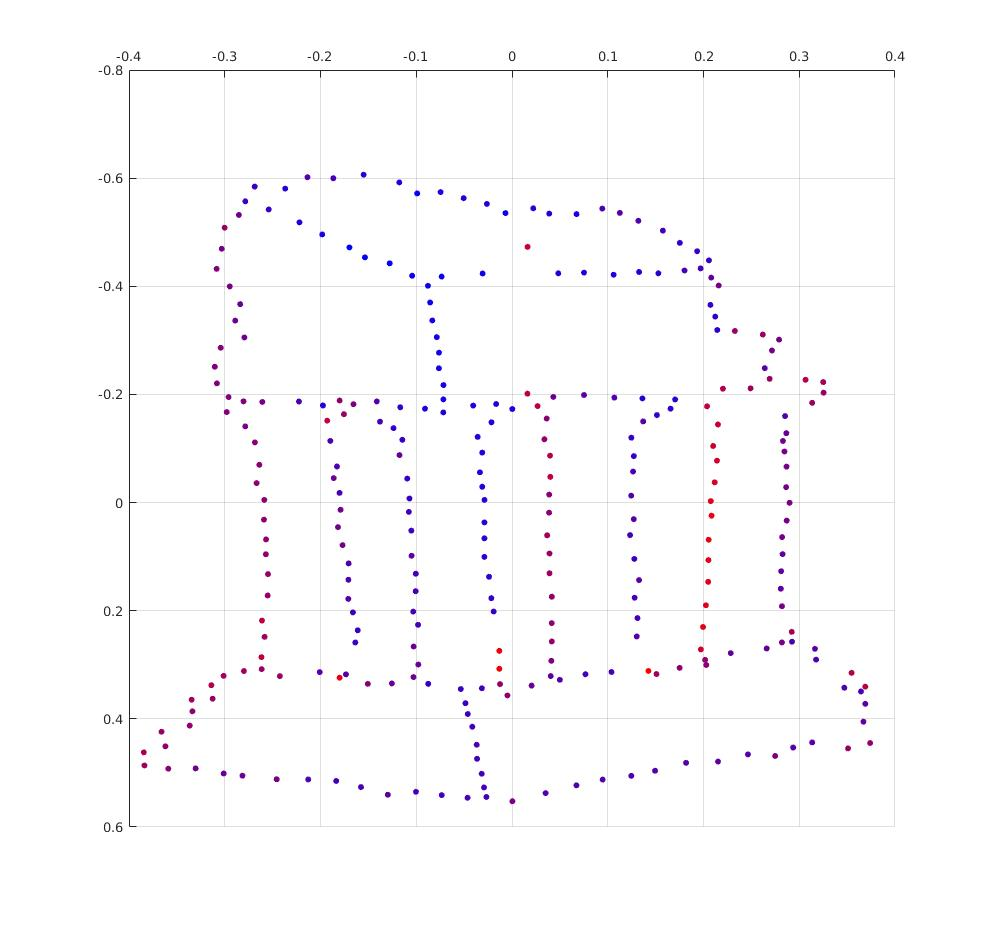
\includegraphics[width=.5\textwidth]{q4_2_2.jpg}} \\
    \subfloat[]{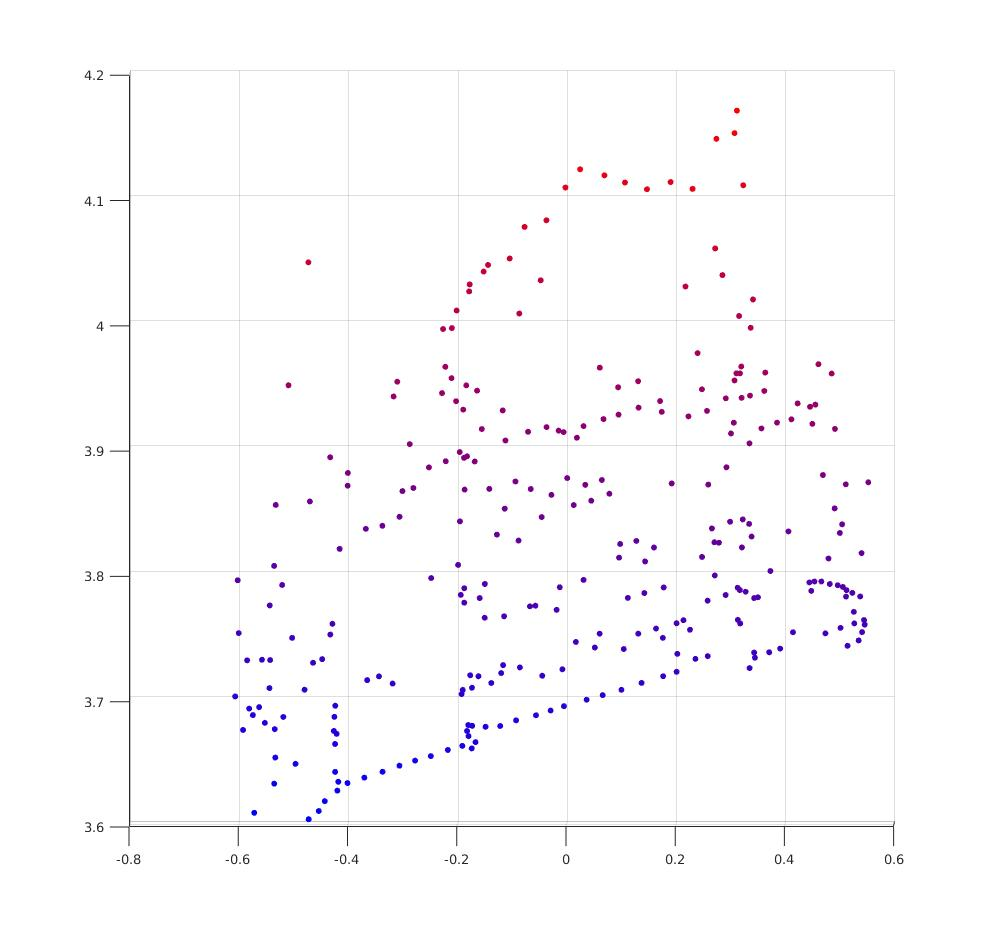
\includegraphics[width=.5\textwidth]{q4_2_3.jpg}} &
    \subfloat[]{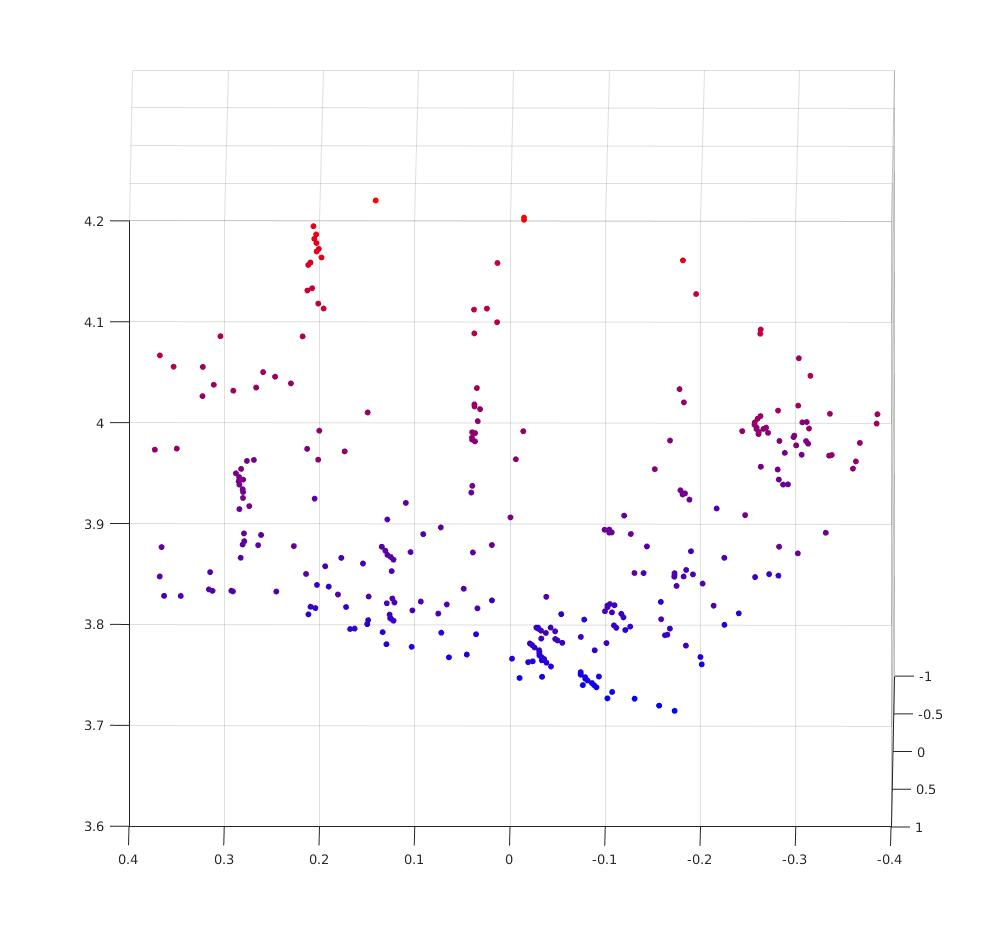
\includegraphics[width=.5\textwidth]{q4_2_4.jpg}} 
\end{tabular}
    \caption{Plots of the system at }
\end{figure}

\end{document}
